\documentclass[a4paper,11pt]{article}
\usepackage[utf8]{inputenc}
\usepackage{graphicx}
\usepackage{enumerate}
\usepackage{geometry}
\usepackage{fancyhdr}
\usepackage{minted}
\usepackage{xcolor}
\usepackage{listings}
\usepackage[colorlinks = true,
            linkcolor = blue,
            urlcolor  = blue,
            citecolor = blue]{hyperref}

\geometry{total={210mm,297mm},
left=25mm,right=25mm,%
bindingoffset=0mm, top=20mm,bottom=20mm}

\graphicspath{ {./images/} }
\renewcommand{\thesubsubsection}{\thesubsection.\alph{subsubsection}}
\renewcommand*\sfdefault{phv}
\renewcommand\familydefault{\sfdefault}

% \renewcommand{\thesubsubsection}{\thesubsection.\alph{subsubsection}}

% \newmintedfile{html}{
%     linenos,
%     breaklines,
%     python3,
%     numbersep=8pt,
%     frame=single,
%     framesep=3mm} 

\newcommand*{\TitleFont}{%
      \usefont{\encodingdefault}{\rmdefault}{b}{n}%
      \fontsize{16}{20}%
      \selectfont}

\linespread{1.3}

% my own titles
\makeatletter
\renewcommand{\maketitle}{
\begin{center}
\vspace{2ex}
{\huge \textsc{\@title}}
\vspace{1ex}
\\
\rule{\linewidth}{0.5pt}\\
\@author \hfill \@date
\vspace{4ex}
\end{center}
}
\makeatother

\definecolor{bg}{rgb}{0.95,0.95,0.95}


% custom footers and headers
\pagestyle{fancy}
\lhead{}
\chead{}
\rhead{}
\lfoot{Assignment 5 : DNSSEC }
\cfoot{}
\rfoot{Page \thepage}
\renewcommand{\headrulewidth}{0pt}
\renewcommand{\footrulewidth}{0pt}
%%----------%%%----------%%%----------%%%----------%%%

\begin{document}

\newminted{bash}{fontsize=\scriptsize, 
    linenos,
    python3,
    numbersep=8pt,
    frame=single,
    bgcolor=bg,
    framesep=3mm} 



% \newminted{all}{linenos, frame=single}

% \usemintedstyle{monokai}
\usemintedstyle{manni}
% \usemintedstyle{xcode}
% \usemintedstyle{vs}
% \usemintedstyle{autumn}
% \usemintedstyle{colorful}
% \usemintedstyle{trac}


\title{ \TitleFont Assignment 5 : DNSSEC }

\author{Emil Sharifulllin, Innopolis University}

\date{\today}

\maketitle

\tableofcontents

\section{Introduction}

\section{Setting Up A Validating Resolver}

\subsection{What does a validating resolver do?}
The job of a validating resolver is to fetch additional information that can be used to computationally verify the answer set. With DNSSEC validation enabled, recursive name servers (validating resolver) will ask for additional resource records in its query, hoping the remote authoritative name servers will respond with more than just the answer to the query, but some proof to go along with the answer as well.

\subsection{Add support for DNSSEC to your BIND or Unbound configuration.}
\subsubsection{What changes do you have to make to your configuration?}
To enable DNSSEC validating resolving in my BIND server I added dnssec-validation auto; to option sector in named.conf.

\begin{bashcode*}{label=/etc/named.conf}
options {
    dnssec-validation auto;
};
\end{bashcode*}

\subsubsection{Verify the root key used against a trusted source.}
To verify BIND root key I compared it with key that is stored at https://www.isc.org/downloads/bind/bind-keys/ and both are the same.

\subsection{How does dig/drill show whether DNSSEC validation was successful or not?}
To check that my DNS server works fine with DNSSEC I ran this command: 
\begin{bashcode}
$ dig @127.0.0.1 www.isc.org. A +dnssec +multiline

; <<>> DiG 9.10.4-P2 <<>> @127.0.0.1 www.isc.org. A +dnssec +multiline
; (1 server found)
;; global options: +cmd
;; Got answer:
;; ->>HEADER<<- opcode: QUERY, status: NOERROR, id: 12344
;; flags: qr rd ra ad; QUERY: 1, ANSWER: 2, AUTHORITY: 5, ADDITIONAL: 8

;; OPT PSEUDOSECTION:
; EDNS: version: 0, flags: do; udp: 4096
;; QUESTION SECTION:
;www.isc.org.		IN A

;; ANSWER SECTION:
www.isc.org.		60 IN A	149.20.64.69
www.isc.org.		60 IN RRSIG A 5 3 60 (
				20161026234027 20160926234027 13953 isc.org.
				O/kgeLanYZuYiUKn8E44Y2sEu0F9Y0e/zQ8zvsjJSkXz
				I77mHbnwIaPeMjNM5wT8nivLi2tQlfo6CX3cBvSR0/6T
				c4eJCJCm0Nsl5Qr+yAnC3DJS5qvQy3gOTdmZEndIMdxC
				D1dopOb95BsjGIniXJcQNP223/RN+f43JSwGdNQ= )

;; AUTHORITY SECTION:
isc.org.		6678 IN	NS ams.sns-pb.isc.org.
isc.org.		6678 IN	NS sfba.sns-pb.isc.org.
isc.org.		6678 IN	NS ns.isc.afilias-nst.info.
isc.org.		6678 IN	NS ord.sns-pb.isc.org.
isc.org.		6678 IN	RRSIG NS 5 2 7200 (
				20161026234027 20160926234027 13953 isc.org.
				BMdkZgZk4Kmn4hIfkFdPlLENE56zdS3lni3G6NI/9u8e
				pUwdYAJ0pjcSEN4EJxXBXkF9OWYqalxsaeAVFbcv3Onj
				0mD5P4ulLWeQsQaaYSixkMfUkY75DvhRQDzluPEa4ELE
				2fk3zxbTTTJ4eR+P1uce9mZOsdcDC7C39xBDizY= )

;; ADDITIONAL SECTION:
ams.sns-pb.isc.org.	85877 IN A 199.6.1.30
ord.sns-pb.isc.org.	85877 IN A 199.6.0.30
sfba.sns-pb.isc.org.	85877 IN A 149.20.64.3
ams.sns-pb.isc.org.	85877 IN AAAA 2001:500:60::30
ord.sns-pb.isc.org.	85877 IN AAAA 2001:500:71::30
sfba.sns-pb.isc.org.	85878 IN AAAA 2001:4f8:0:2::19
sfba.sns-pb.isc.org.	6678 IN	RRSIG AAAA 5 4 7200 (
				20161026234027 20160926234027 13953 isc.org.
				Amoqjz/z16YrO/NLX3C9cx9kPJ0tMmoBWUjfwuiQedmp
				77dOjUB9IFhgscRn35xFEUket4vFMtJ7PyUdNYtf3x1I
				UYoX6JeYjI4m/TYwYoH5yQCRG9xJbtzqki+2AnR1hL14
				UPDFACa1s2OdSgF8j/evQ5QTcRN6hHJ4IbvjIxI= )

;; Query time: 209 msec
;; SERVER: 127.0.0.1#53(127.0.0.1)
;; WHEN: Tue Sep 27 14:57:00 MSK 2016
;; MSG SIZE  rcvd: 788
\end{bashcode}

\begin{bashcode}
$ dig @127.0.0.1 www.os3.nl. A +dnssec +multiline 

; <<>> DiG 9.10.4-P2 <<>> @127.0.0.1 www.os3.nl. A +dnssec +multiline
; (1 server found)
;; global options: +cmd
;; Got answer:
;; ->>HEADER<<- opcode: QUERY, status: NOERROR, id: 62627
;; flags: qr rd ra ad; QUERY: 1, ANSWER: 2, AUTHORITY: 0, ADDITIONAL: 1

;; OPT PSEUDOSECTION:
; EDNS: version: 0, flags: do; udp: 4096
;; QUESTION SECTION:
;www.os3.nl.		IN A

;; ANSWER SECTION:
www.os3.nl.		21600 IN A 145.100.96.70
www.os3.nl.		21600 IN RRSIG A 5 3 21600 (
				20161027115344 20160927115344 42048 os3.nl.
				k61oLlNtqIPLEF0cjvqu5tBOr7aElawOYHDrvtlQNxlo
				6Tf5BPnzcI9nNhXzpw2coNDnadxaNmRAfWt6KIZurAoS
				TC6mZjcTwcnk5HDQff19MN3rcqiwt7TSwJyST4HLRIan
				Jm4muRcdsN1ocB2PK1u6qUHd7MiDgZ8LH9AMBcA= )

;; Query time: 855 msec
;; SERVER: 127.0.0.1#53(127.0.0.1)
;; WHEN: Tue Sep 27 16:53:10 MSK 2016
;; MSG SIZE  rcvd: 221

\end{bashcode}

As we can see recursor replied us with flag AD which means that dig used DNSSEC for this request. Also our server responded to us with status: NOERROR and it means that validity done.\\
We also can check that for domains with bad validity dig will report SERVFAIL.

\begin{bashcode}
$ dig @127.0.0.1  www.dnssec-failed.org. A +dnssec +multiline 

; <<>> DiG 9.10.4-P2 <<>> @127.0.0.1 www.dnssec-failed.org. A +dnssec +multiline
; (1 server found)
;; global options: +cmd
;; Got answer:
;; ->>HEADER<<- opcode: QUERY, status: SERVFAIL, id: 22227
;; flags: qr rd ra; QUERY: 1, ANSWER: 0, AUTHORITY: 0, ADDITIONAL: 1

;; OPT PSEUDOSECTION:
; EDNS: version: 0, flags: do; udp: 4096
;; QUESTION SECTION:
;www.dnssec-failed.org.	IN A

;; Query time: 3167 msec
;; SERVER: 127.0.0.1#53(127.0.0.1)
;; WHEN: Tue Sep 27 16:55:41 MSK 2016
;; MSG SIZE  rcvd: 50	
\end{bashcode}

\subsection{Where does BIND/Unbound store the DNSSEC root key?}
DNSSEC root key for BIND is stored in /etc/bind.keys

\begin{bashcode*}{label=/etc/bind.keys}
/* $Id: bind.keys,v 1.7 2011/01/03 23:45:07 each Exp $ */
# The bind.keys file is used to override the built-in DNSSEC trust anchors
# which are included as part of BIND 9.  As of the current release, the only
# trust anchors it contains are those for the DNS root zone ("."), and for
# the ISC DNSSEC Lookaside Validation zone ("dlv.isc.org").  Trust anchors
# for any other zones MUST be configured elsewhere; if they are configured
# here, they will not be recognized or used by named.
#
# The built-in trust anchors are provided for convenience of configuration.
# They are not activated within named.conf unless specifically switched on.
# To use the built-in root key, set "dnssec-validation auto;" in
# named.conf options.  To use the built-in DLV key, set
# "dnssec-lookaside auto;".  Without these options being set,
# the keys in this file are ignored.
#
# This file is NOT expected to be user-configured.
#
# These keys are current as of January 2011.  If any key fails to
# initialize correctly, it may have expired.  In that event you should
# replace this file with a current version.  The latest version of
# bind.keys can always be obtained from ISC at https://www.isc.org/bind-keys.

managed-keys {
	# ISC DLV: See https://www.isc.org/solutions/dlv for details.
        # NOTE: This key is activated by setting "dnssec-lookaside auto;"
        # in named.conf.
	dlv.isc.org. initial-key 257 3 5 "BEAAAAPHMu/5onzrEE7z1egmhg/WPO0+juoZrW3euWEn4MxDCE1+lLy2
		brhQv5rN32RKtMzX6Mj70jdzeND4XknW58dnJNPCxn8+jAGl2FZLK8t+
		1uq4W+nnA3qO2+DL+k6BD4mewMLbIYFwe0PG73Te9fZ2kJb56dhgMde5
		ymX4BI/oQ+cAK50/xvJv00Frf8kw6ucMTwFlgPe+jnGxPPEmHAte/URk
		Y62ZfkLoBAADLHQ9IrS2tryAe7mbBZVcOwIeU/Rw/mRx/vwwMCTgNboM
		QKtUdvNXDrYJDSHZws3xiRXF1Rf+al9UmZfSav/4NWLKjHzpT59k/VSt
		TDN0YUuWrBNh";

	# ROOT KEY: See https://data.iana.org/root-anchors/root-anchors.xml
	# for current trust anchor information.
        # NOTE: This key is activated by setting "dnssec-validation auto;"
        # in named.conf.
	. initial-key 257 3 8 "AwEAAagAIKlVZrpC6Ia7gEzahOR+9W29euxhJhVVLOyQbSEW0O8gcCjF
		FVQUTf6v58fLjwBd0YI0EzrAcQqBGCzh/RStIoO8g0NfnfL2MTJRkxoX
		bfDaUeVPQuYEhg37NZWAJQ9VnMVDxP/VHL496M/QZxkjf5/Efucp2gaD
		X6RS6CXpoY68LsvPVjR0ZSwzz1apAzvN9dlzEheX7ICJBBtuA6G3LQpz
		W5hOA2hzCTMjJPJ8LbqF6dsV6DoBQzgul0sGIcGOYl7OyQdXfZ57relS
		Qageu+ipAdTTJ25AsRTAoub8ONGcLmqrAmRLKBP1dfwhYB4N7knNnulq
		QxA+Uk1ihz0=";
};
	
\end{bashcode*}

\subsection{How do “managed keys” differ from “trusted keys”? Which RFC describes the mechanisms for managedkeys?}
Managed keys is the keys that is updated automatically by DNS server. Trusted keys is a keys that is defined manually. The RFC that describes keys management is a \href{https://tools.ietf.org/html/rfc5011}{RFC 5011 - Automated Updates of DNS Security (DNSSEC) Trust Anchors} Trusted keys is very useful

\subsection{How did you modify the DNSSEC root key?}
To modify BIND root key I modified file /etc/bind.keys section root key.

Here you can see t

\subsection{What problems did your server encounter, and how did it react?}
After changing of root key I created new dns request with dig and in response gone AD flag.
\begin{bashcode}
$ dig @127.0.0.1 www.isc.org. A +dnssec +multiline

; <<>> DiG 9.10.4-P2 <<>> @127.0.0.1 www.isc.org. A +dnssec +multiline
; (1 server found)
;; global options: +cmd
;; Got answer:
;; ->>HEADER<<- opcode: QUERY, status: NOERROR, id: 48579
;; flags: qr rd ra; QUERY: 1, ANSWER: 2, AUTHORITY: 4, ADDITIONAL: 6

;; OPT PSEUDOSECTION:
; EDNS: version: 0, flags: do; udp: 4096
;; QUESTION SECTION:
;www.isc.org.		IN A

;; ANSWER SECTION:
www.isc.org.		60 IN A	149.20.64.69
www.isc.org.		60 IN RRSIG A 5 3 60 (
				20161026234027 20160926234027 13953 isc.org.
				O/kgeLanYZuYiUKn8E44Y2sEu0F9Y0e/zQ8zvsjJSkXz
				I77mHbnwIaPeMjNM5wT8nivLi2tQlfo6CX3cBvSR0/6T
				c4eJCJCm0Nsl5Qr+yAnC3DJS5qvQy3gOTdmZEndIMdxC
				D1dopOb95BsjGIniXJcQNP223/RN+f43JSwGdNQ= )

;; AUTHORITY SECTION:
isc.org.		86400 IN NS sfba.sns-pb.isc.org.
isc.org.		86400 IN NS ord.sns-pb.isc.org.
isc.org.		86400 IN NS ams.sns-pb.isc.org.
isc.org.		86400 IN NS ns.isc.afilias-nst.info.

;; ADDITIONAL SECTION:
ams.sns-pb.isc.org.	86400 IN A 199.6.1.30
ord.sns-pb.isc.org.	86400 IN A 199.6.0.30
sfba.sns-pb.isc.org.	86400 IN A 149.20.64.3
ams.sns-pb.isc.org.	86400 IN AAAA 2001:500:60::30
ord.sns-pb.isc.org.	86400 IN AAAA 2001:500:71::30

;; Query time: 390 msec
;; SERVER: 127.0.0.1#53(127.0.0.1)
;; WHEN: Wed Sep 28 14:13:16 MSK 2016
;; MSG SIZE  rcvd: 426
\end{bashcode}

\section{Setting Up A Secure Zone}
\addtocounter{subsection}{8}
\subsection{Look up which cryptographic algorithms are available for use in DNSSEC. Which one do you prefer, and why?}
DNSSEC can work with nine cryptograpfic algorithms:

\begin{center}
\begin{tabular}{|c|c|c|c|}
\hline
Algorithm field & Algorithm & Source & Implementation status \\ \hline\hline
1 & RSA/MD5 & - & Must Not Implement \\ \hline
3 & DSA/SHA-1 & - & Optional \\ \hline
5 & RSA/SHA-1 & RFC 3110 & Required \\ \hline
7 & RSASHA1-NSEC3-SHA1 & RFC 5155 &	Recommended \\ \hline
8 & RSA/SHA-256 & RFC 5702 & Recommended \\ \hline
10 & RSA/SHA-512 & RFC 5702 & Recommended \\ \hline
12 & GOST R 34.10-2001 & RFC 5933 & Optional \\ \hline
13 & ECDSA/SHA-256 & RFC 6605 & Recommended \\ \hline
14 & ECDSA/SHA-384 & RFC 6605 & Recommended \\ \hline
\end{tabular}
\end{center}
To choose algorithm I dcided between those which only have required ot recommended status. In following papers is described why I should to use MD5, 1024 bit RSA and SHA1:
\begin{itemize}
	\item \href{http://www.kb.cert.org/vuls/id/836068}{MD5 vulnerable to collision attacks}
	\item \href{http://arstechnica.com/uncategorized/2007/05/researchers-307-digit-key-crack-endangers-1024-bit-rsa/}{307-digit key crack endangers 1024-bit RSA}
	\item \href{https://www.schneier.com/blog/archives/2012/10/when_will_we_se.html}{When Will We See Collisions for SHA-1?}
\end{itemize}
In this case I chose RSASHA256 as a main cryptographic algorithm.

\subsection{In practice, different algorithms, key sizes and key lifetimes are chosen for KSKs and ZSKs. Discuss what are these differences in:}
The main difference in KSK and ZSK is that zones is needed to be resigned every time when zone changes and KSK is KSK used only when ZSK changed.
\subsubsection{algorithms}
For DNSSEC there is not important that KSK ans ZSK is signed with same or different algorithms so you can choose both variants.
\subsubsection{key sizes} ZSK should have lower size than KSK to reduce server load because zones must to be resigned every time they changed. KSK is needed to have greater length because it should have higher security than ZSK.
\subsubsection{key lifetimes}
It's necessary to change ZSK more frequent than KSK because it usually have lower key size and it's easy to find private key for it. KSK usually have higher key length and every time when it changed it's hash must be sent to parent zone server so KSK should be changed less frequently

\subsection{Choose appropriate algorithms, key sizes and key lifetimes for your KSK and ZSK.}
For my zone I chose following configurations: 
\begin{itemize}
	\item \textbf{KSK:} RSASHA256, 2048 bits, 1 year
	\item \textbf{ZSK:} RSASHA256, 1024 bits, 3 months
\end{itemize}

\subsection{Show the signed version of your zone file. How does it differ from the unsigned version? Any unexpecteddifferences?}
To generate keys I ran following commands:
\begin{bashcode}
$  sudo mkdir -p /etc/named/keys/st10.os3.su
$  ~  cd /etc/named/keys/st10.os3.su 
$ dnssec-keygen -a RSASHA256 -b 1024 st10.os3.su
Generating key pair................++++++ ........................................++++++ 

$ sudo dnssec-keygen -a RSASHA256 -b 2048 -f KSK st10.os3.su
Generating key pair...........................+++ .+++ 
Kst10.os3.su.+008+50107
\end{bashcode}
In BIND config file I added settings to add this zone signing and reloaded named.

\begin{bashcode*}{label=/etc/named.conf}
zone "st10.os3.su." {
        type master;
        file "st10.os3.su.zone";
        key-directory "keys/st10.os3.su";
        inline-signing yes;
        auto-dnssec maintain;
};
\end{bashcode*}
After this in /etc/named created new binary file called st10.os3.su.zone.signed that is signed zone file so now we can check validity of our dns zone.

\begin{bashcode}
delv @127.0.0.1 -a /tmp/st10.os3.su +root=st10.os3.su st10.os3.su. SOA +multiline
; fully validated
st10.os3.su.		86400 IN SOA ns10.os3.su. admin.st10.os3.su. (
				2016082905 ; serial
				360000     ; refresh (4 days 4 hours)
				3600       ; retry (1 hour)
				3600000    ; expire (5 weeks 6 days 16 hours)
				3600       ; minimum (1 hour)
				)
st10.os3.su.		86400 IN RRSIG SOA 8 3 86400 (
				20161028141048 20160928131048 57405 st10.os3.su.
				coN0g1MLy7KZQKsHfGqFyazqC3cVLCHhgCIzDxINjrlS
				fSFNUNLVRq+Yl+m/7D8BIQtTD+eELKD4nfr1rR+vFJfQ
				puSI7gdiuR273kuVUaChW2KWGbeYor1DTOD7yw0tNqbL
				cc/wEqsjf2OrBH44BRgm3LkDvBQirH4JRbdRZbA= )	
\end{bashcode}

\subsection{Which DS record do you need to send to your neighbors, and why that one?}
I need to send DS record of KSK of zone st10.st11.os3.su to my neighbour. He must to add this DS records to him st11.os3.su. zone file. To generate DS record I used
\begin{bashcode}
$ dnssec-dsfromkey -a SHA-1 Kst10.st11.os3.su.+008+49704.key 
st10.st11.os3.su. IN DS 49704 8 1 76BE781D1D1C3D672AFEFA0736694138F7EB3611

$ dnssec-dsfromkey -a SHA-256 Kst10.st11.os3.su.+008+49704.key 
st10.st11.os3.su. IN DS 49704 8 2 1DD63C458BDC1036CF6B6A1D32A55634AB9F5A2043A590005E280A8DDD9495D6
\end{bashcode}

\subsection{Show the results of the examination of your secured domain.}
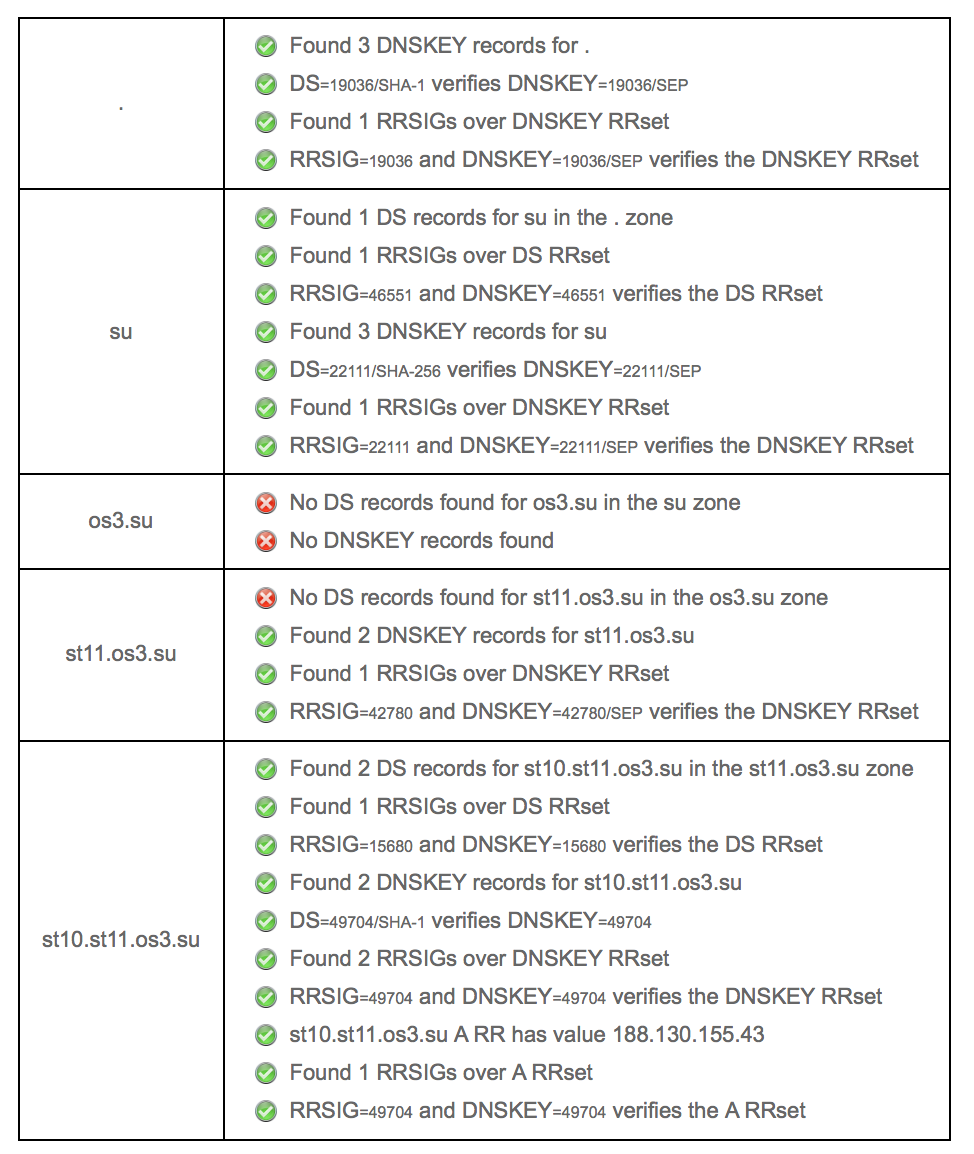
\includegraphics{zone-verification}

\subsection{Describe which DS and DNSKEY records are important for your domain. Which keys are used where?}
In my case there are two DS records for only one domain and they are most important for me.

\begin{bashcode*}{label=My DS records}
st10.st11.os3.su. IN DS 49704 8 1 76BE781D1D1C3D672AFEFA0736694138F7EB3611
st10.st11.os3.su. IN DS 49704 8 2 1DD63C458BDC1036CF6B6A1D32A55634AB9F5A2043A590005E280A8DDD9495D6
\end{bashcode*}
Both of DNSKEY records is very important for security because if any of private key will leak advisor can spoof our zone.

\section{Key Rollovers}
\addtocounter{subsection}{15}
\subsection{Start planning for a Zone Signing Keyrollover.}
\subsubsection{Describe the options for doing a ZSK rollover, make a motivated choice for one procedure.}
DNSSEC rollover can be made in two ways: Pre-publication and Double Signature. Pre-publication is slower but zone file will not increase very. Double Signature is quicker but increases zone file size. I chose pre-publication way.
\subsubsection{How do you implement this procedure with the tools for signing your zone?}
I made ZSK rollover for my zone st10.os3.su. before rollover my zone key was 57405, after rollover it was ****. To make this process I used following commands
\begin{bashcode}
$ cd /etc/named/keys/st10.os3.su
$ sudo dnssec-settime -I 20160929234000 -D 20161029 Kst10.os3.su.+008+57405
$ sudo dnssec-keygen -i 10 -S Kst10.os3.su.+008+57405 
Generating key pair......++++++ .++++++ 
Kst10.os3.su.+008+14889
\end{bashcode}
After this steps key rollover will be made at Thu Sep 29 23:40:00 2016

\subsubsection{Which timers are important for this procedure?}
For key rollover important is \textbf{Inactive} timers which say when time of inactivating is gone BIND will not accept this key for signing. Second timer is \textbf{Delete} timer which says to BIND when to delete inactive key file.
\subsubsection{Implement the procedure and use a DNSSEC debugger to verify each step. Don’t forget to show the results of each verification.}

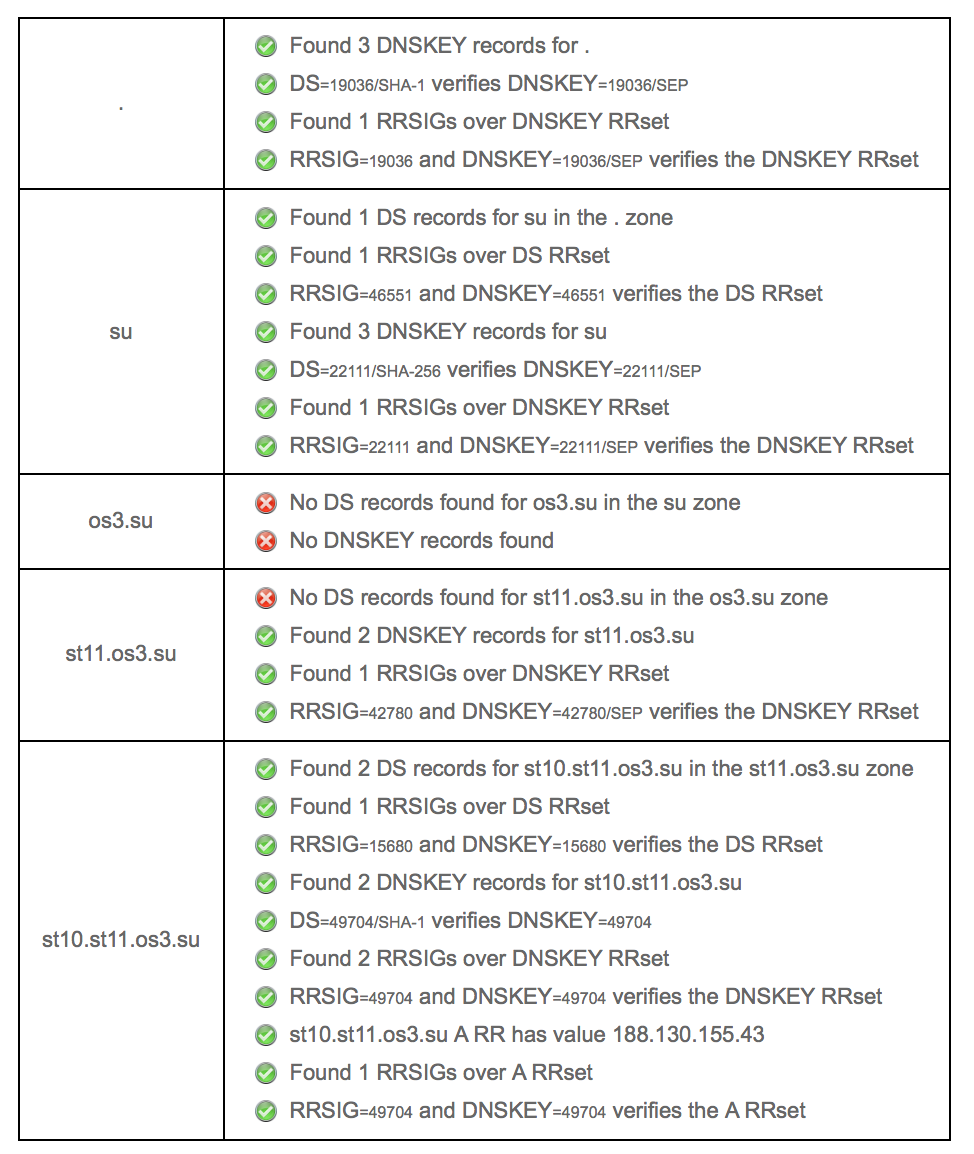
\includegraphics{after}

\subsection{Can you use the same procedure for a KSK rollover? What does this depend on?}
KSK rollover is very similar to ZSK, with the addition of interacting with the parent zone. When the child zone wants to roll, it notifies the parent during the "new DS" phase and submits the new key. As said in RFC 4641: \\
During the rollover ("new DNSKEY" phase),
   which can take place as soon as the new DS set propagated through the
   DNS, the child replaces DNSKEY1 with DNSKEY2.  Immediately after that
   ("DS/DNSKEY removal" phase), it can notify the parent that the old DS
   record can be deleted.
   The drawbacks of this scheme are that during the "new DS" phase the
   parent cannot verify the match between the DS2 RR and DNSKEY2 using
   the DNS -- as DNSKEY2 is not yet published.  Besides, we introduce a
   "security lame" key (see Section 4.4.3).  Finally, the child-parent
   interaction consists of two steps.  The "double signature" method
   only needs one interaction.
\end{document}